
%%%%%%%%%%%%%%%%%%%%%%% file typeinst.tex %%%%%%%%%%%%%%%%%%%%%%%%%
%
% This is the LaTeX source for the instructions to authors using
% the LaTeX document class 'llncs.cls' for contributions to
% the Lecture Notes in Computer Sciences series.
% http://www.springer.com/lncs       Springer Heidelberg 2006/05/04
%
% It may be used as a template for your own input - copy it
% to a new file with a new name and use it as the basis
% for your article.
%
% NB: the document class 'llncs' has its own and detailed documentation, see
% ftp://ftp.springer.de/data/pubftp/pub/tex/latex/llncs/latex2e/llncsdoc.pdf
%
%%%%%%%%%%%%%%%%%%%%%%%%%%%%%%%%%%%%%%%%%%%%%%%%%%%%%%%%%%%%%%%%%%%


\documentclass[runningheads,a4paper]{llncs}

\usepackage{amssymb}
\setcounter{tocdepth}{3}
\usepackage{graphicx}
\usepackage{float}
\usepackage[full]{complexity}
\usepackage{amsmath}
%\usepackage{amsfonts}
%\usepackage{amsthm}
\usepackage{subfigure}
%\usepackage{caption}
%\usepackage{subcaption}
%\usepackage{cite}
\usepackage{hyperref}
\usepackage{url}
%\usepackage{clrscode4e}
\usepackage{verbatim}
\urlstyle{same}
\newcommand{\keywords}[1]{\par\addvspace\baselineskip
\noindent\keywordname\enspace\ignorespaces#1}
\newcommand{\QSAT}{\mathsf{QSAT}}
\newcommand{\UQSAT}{\mathsf{UQSAT}}

% Uniform numbering for previously defined theorem environments (e.g., LNCS).
\makeatletter
\let\c@lemma=\c@theorem
\let\c@corollary=\c@theorem
\let\c@fact=\c@theorem
\makeatother

% Redefinition of LNCS or SODA or Springer proof environment to put a \Box at
% the end of every proof.
\let\realendproof=\endproof
\def\endproof{\hspace*{\fill}$\Box$\realendproof}

\begin{document}

\mainmatter  % start of an individual contribution

% first the title is needed
\title{The Fewest Clues Problem}

% a short form should be given in case it is too long for the running head
\titlerunning{The Fewest Clues Problem}

% the name(s) of the author(s) follow(s) next
%
% NB: Chinese authors should write their first names(s) in front of
% their surnames. This ensures that the names appear correctly in
% the running heads and the author index.
%
\author{Erik D. Demaine \and Fermi Ma \and Ariel Schvartzman \and Erik Waingarten}
%
\authorrunning{Fermi Ma \and Ariel Schvartzman \and Erik Waingarten}
% (feature abused for this document to repeat the title also on left hand pages)

% the affiliations are given next; don't give your e-mail address
% unless you accept that it will be published
\institute{MIT,\\
77 Mass Ave., Cambridge, MA 02139, USA, \\
\protect\url{{edemaine,fermima,arielsc,eaw}@mit.edu}}

%
% NB: a more complex sample for affiliations and the mapping to the
% corresponding authors can be found in the file "llncs.dem"
% (search for the string "\mainmatter" where a contribution starts).
% "llncs.dem" accompanies the document class "llncs.cls".
%

\maketitle

\begin{abstract}
We study the problem of finding the fewest number of clues needed for a particular puzzle to be unique. We define a general transformation from search problems to fewest clues problems. We explore how the computational complexity of the problems change when we apply the transformation. We define two types of reductions relating fewest clues problems, and we show various \NP-complete problems have fewest clues versions which are $\Sigma_2$-complete. This line of research is similar to exploring the power of counting, as in \#P and ASP (another solution problem).
\end{abstract}

\section{Introduction}
\label{sec:introduction}

The difficulty of many pencil and paper puzzles is closely correlated with the number of clues or hints given. A standard example of this is the famous Sudoku puzzle, where the puzzle solver is given a $9 \times 9$ subgrid divided into nine $3 \times 3$ subgrids, along with certain squares of the puzzle filled in with digits. The goal is to fill in each square of the grid with digits so that each of row, column, and each of the nine $3 \times 3$ subgrids contains all the digits. Sudoku puzzles are usually required to be uniquely solvable given the initial clues.

In 2012, McGuire, Tugermann, and Civario confirmed the long-standing conjecture that there are no uniquely solvable 16-clue Sudoku puzzles \cite{mcguire2012there}. On the other hand, there exists an online database with over 50,000 uniquely solvable 17-clue Sudoku puzzles. Thus, McGuire et al. completely solved the problem of finding the fewest number of clues necessary to solve a Sudoku. However, their result followed from a year-long computation, prompting the question: for what other problems is it hard to determine the fewest number of necessary clues?

In this paper, we focus on asking this fewest clues question for problems in $\mathsf{NP}$, where ``clues" are fragments of problem solutions. For example, if the problem is to find a Hamiltonian cycle in a given graph, our question would be to determine the minimum number of graph edges (clues) that must be specified such that exactly one Hamiltonian cycle contains all the  specify before only one Hamiltonian cycle contains all specified edges. We call this the ``Fewest Clues Problem" ($\mathsf{FCP}$) and we treat $\mathsf{FCP}$ as a transformation of problems. 

\subsection{Definitions}

For a given instance of $x$ of an $\NP$ \emph{search} problem A, the solutions to $x$ can be written as polynomial-length strings. Consider the boolean satisfiability problem ($\SAT$), where an instance consists of a specific $\SAT$ formula on variables $x_1,\dots,x_n$. Solutions can be written as indexed length-$n$ strings of Boolean values, where the value at index $i$ is the assignment to variable $x_i$. A $\emph{clue}$ for the problem would be an assignment of a specific index to some Boolean value. For general problems, the precise definition of a clue depends on how solutions are encoded as strings.

We say that a solution to $x$ \emph{satisfies} a set of clues if each clue matches the solution at that clue's index. For example, in the case of SAT on variables $x_1,x_2,\dots,x_5$, the solution $``01011"$ matches the clue set $\{x_1 = 0,x_3 = 0,x_4 = 1\}$.

We now define $\mathsf{FCP} A$ to be the following decision problem:
\begin{quote}
Given $A$ and a valid encoding of solutions of $A$, is there a set of at most $k$ clues such that exactly one solution satisfies these clues?
\end{quote}
%
%In particular, we will have an $\NP$ search problem be comprised of a set of \emph{instances}, which will be strings over some finite alphabet. For a particular instance $x$, there is set of possible \emph{solutions}, which are strings of polynomial size with respect to $|x|$ over some finite alphabet. Each problem also comes with an algorithm $A$ that checks whether a string $s$ is in fact a solution for an instance $x$, which runs in polynomial time. This is the verifier. For a given language $L \in \NP$, $x \in L$ if and only if $S(x)$ is non-empty.
%
%A \emph{clue} will be an indexed character of a solution. So a clue indicates what character lies at some position of the solution.
%
%\begin{definition}
%Given some $\NP$ search problem $A$, the ``fewest clues" version of $A$, $(\mathsf{FCP} A)$ asks for an instance of $A$, the minimum number of clues corresponding to a unique solution for any given instance?
%\end{definition}

As an example, consider the classical $9 \times 9$ Sudoku. We write solutions as strings of length 81 with the alphabet $\Sigma = \{ 1, ..., 9 \} \cup \{ \Box \}$, where each position in the string corresponds to a position on the $9 \times 9$ Sudoku board. The presence of a $\Box$ indicates an empty square. In $\mathsf{FCP}$ Sudoku, the instance is a given 81 character string $x$ that contains some number of empty squares. The problem is to find the fewest number of additional squares that must be filled for the Sudoku to be uniquely solvable. Thus, the problem of determining the fewest number of clues necessary for a Sudoku puzzle is the $\mathsf{FCP}$ Sudoku problem where $x$ is the empty strings of all $\Box$ characters.

%
%We use this framework to analyze the $\mathsf{FCP}$ versions of classic $\NP$-hard problems, and we find that for many $\NP$-hard problems, their $\mathsf{FCP}$ versions are $\Sigma_2$-complete. We also consider $\mathsf{FCP}$ version of problems in $P$, and find comp
%
%
% such as SAT and 3SAT, as well as $\NP$-hard puzzle problems such as Latin Square completion and Sudoku completion. We show that for many $\NP$-hard problems, their $\mathsf{FCP}$ versions are $\Sigma_2$-complete, and give examples of problems with polynomial time algorithms whose $\mathsf{FCP}$ versions are $\Sigma_2$-complete.
%
%The paper is organized as follows. In Section~\ref{sec:relatedwork}, we discuss previous research done on this problem for the specific cases of Sudoku, Latin Squares, and graph coloring. We note that while fewest clues problems has been studied extensively, it is almost always done so with respect to a certain problem. In Section~\ref{sec:prelim}, we motivate and formally define the transformation $\mathsf{FCP}$. We state what it means for a problem to be a fewest clues problem, and provide a framework for reducing between these problems. In Section~\ref{sec:The Problems}, we consider $\mathsf{FCP}$ versions of the SAT, 3SAT, Triangle Partition, Latin Squares and Sudoku completion problems, and show why these problems are $\Sigma_2$-complete. Then in Section~\ref{sec:easyproblems} we discuss how the $\mathsf{FCP}$ transformation affects problems with polynomial time algorithms. Finally, in Section~\ref{sec:conclusion} we give concluding remarks and ideas for further research.

\subsection{Related Work}
\label{sec:relatedwork}

Our work touches upon three major areas: critical sets, Boolean formula minimization, and the Another Solution Problem (ASP) \

\noindent\textbf{Critical Sets.} A critical set is another name for minimum clue sets \cite{Cooper:2014:CSS:2612293.2612628}. However, there is very little work on the general problem of finding critical sets for $\NP$ search problems. Prior work on critical sets tends to focus on the critical set problem for specific $\NP$ search problems.

Previous work by \cite{Cooper:2014:CSS:2612293.2612628} studies the problem of finding critical sets in Sudoku puzzles by relating the problem to graph colorings. Their approach is to view Sudoku puzzles as graphs by transforming each grid square into a node and edges between vertices whose corresponding squares cannot contain the same number. An $n$-coloring of the graph then corresponds to a solution to the Sudoku. Therefore, finding the fewest number of vertices to color so that the remaining graph has a unique $n$-coloring is equivalent to finding a critical set for the Sudoku. They prove an $\NP$-hardness result for the problem of determining critical sets for graph coloring. In this paper, we improve their result and show a $\Sigma_2$-completeness result for this problem.
%
%Another line of research which is also very similar has been that of determining the size of critical sets. \cite{Cooper:2014:CSS:2612293.2612628} defines critical sets in much the same way we do; determining the fewest number of clues needed to obtain a unique solution. They focus on colorings on graphs. They can think of the Sudoku puzzle as a graph. This is a graph with $n^2$ vertices (one for each square), which has edges between vertices whose corresponding squares cannot be the same values. They ask for the smallest number of vertices needed to color in order for the remaining graph to have a unique $n$ color coloring. This is phrasing the problem of \cite{mcguire2012there} in graph and coloring notation. 
%
%They prove some results regarding the sizes of critical sets for graph colorings and show that the problem is $\NP$-hard. Our results improve on these results by showing that these graph colorings are in fact $\Sigma_2$-complete, which fully characterizes their complexity.

\noindent\textbf{Boolean Formula Minimization}. Our approach to showing $\Sigma_2$-hardness of Boolean formula minimization has many connections to Boolean formula minimization. \cite{umans}\cite{umans2001minimum} explores the problem of Minimum Equivalent Expression and Shortest Implicant. The problem is very similar to the problem we consider when applied to SAT. In the Shortest Implicant problem, they ask for the minimum number of variables needed so that the formula is always satisfiable, no matter what assignment the other variables receive. They show this problem is $\Sigma_2$-complete.  \\

\noindent\textbf{The Another Solution Problem ($\mathsf{ASP}$)}. Our approach the $\mathsf{FCP}$ transformation is related to the \emph{Another Solution Problem} ($\mathsf{ASP}$) \cite{Seta01}. For a given problem, the $\mathsf{ASP}$ version asks: given an instance and a solution for that instance, find another solution for that instance. There is a notion of an $\mathsf{ASP}$-reduction, defined in \cite{Seta01}. If $\mathsf{ASP} A$ can be $\mathsf{ASP}$-reduced to $\mathsf{ASP} B$, then $\mathsf{NP}$-hardness of $\mathsf{ASP} A$ implies $\mathsf{NP}$-hardness of $\mathsf{ASP} B$. In a follow-up paper, \cite{takayuki2003complexity} shows $\mathsf{ASP}$-completeness of Slither Link, Sudoku (or Number Place), and Fillomino. We use a similar approach to analyzing hardness of $\mathsf{FCP}$-hard problems. 

We consider the $\mathsf{FCP}$ version of the Boolean satisfiability problem ($\SAT$), and show that it is $\Sigma_2$-complete. We then define an $\mathsf{FCP}$-reduction similar in flavor to an $\mathsf{ASP}$-reduction, and show $\Sigma_2$-completenss of various $\mathsf{FCP}$ problems with these reductions.\\


\cite{Ghandehari2005121} did a similar type of analysis, where they bound the size of the smallest critical set for Latin Squares. \cite{1984computational} also analyzes the complexity of recognizing critical sets. They ask exactly the ASP question for Latin Squares, and show it is $\NP$-complete.


\section{The $\mathsf{FCP}$ Transformation}
\label{sec:prelim}

\subsection{Upper Bounds}

Usually, we will study problems in $\NP$ and their $\mathsf{FCP}$ transformation.

\begin{theorem}
\label{thm:satinsig2}
If $L \in \NP$, then $\mathsf{FCP} L \in \Sigma_2^P$. 
\end{theorem}

\begin{proof}
We will write $\mathsf{FCP} L$ in terms of a $\Sigma_2^P$ question. The original $\NP$ question for $L$ is
\[ x \in L \leftrightarrow \exists y, A(x, y) = 1, \]
where $A$ is a polynomial time algorithm and the length of $y$ is some polynomial in the length of $x$. Alternatively, we think of the relation $R = \{ (x, y) | A(x,y) = 1 \}$. Then, $L = \{ x | (x,y) \in R \}$. 

The $\NP$ question for $L$ asks: for some given $x$, does there exists some $y$ such that $(x, y) \in R$?

$\mathsf{FCP} L$ asks: for some given $x$ and $k$, does there exists at most $k$ indexed characters, $c_y$, such that only one $y$ with $c_y \subset y$ has $(x,y) \in R$. 

In logical notation, the $\mathsf{FCP} L$ question is
\[ (x, k) \in \mathsf{FCP} L \leftrightarrow \exists c_y, y \forall y' A'(x, c_y, y, y') = 1. \]
The algorithm $A'$ checks the following:
\begin{itemize}
\item $c_y \subset y$, $|c_y| \leq k$
\item $c_y \subset y' \neq y$ 
\item $A(x,y) = 1$
\item $A(x, y') = 0$ 
\end{itemize}
$c_y$ contains the clues for $y$. $y'$ is another solution. $A'$ checks $c_y$ has at most $k$ elements, that it is a clue of the solution $y$, and that there are no other solutions.
\end{proof}

We could generlize Theorem~\ref{thm:satinsig2}. The proof of Theorem~\ref{thm:satinsig2} proves the following claim.
\begin{claim} If $L \in \NTIME[f(n)]$, then $\mathsf{FCP} L \in \Sigma_2 \NTIME[f(n)]$, when $f(n) > n$.
\end{claim}

\subsection{$\mathsf{FCP} \SAT$}

We define $\mathsf{FCP} \SAT$. This will be the first $\mathsf{FCP}$ problem which is $\Sigma_2^P$-complete. 

\vbox{%
\noindent
\textsc{$\mathsf{FCP} \SAT$}
\begin{quote}
\begin{description}
\item[Instance:] A Boolean formula $\phi$, and a number $k$.
\item[Question:] Does there exists a partial assignment of at most $k$ variables such that the remaining formula $\phi'$ has only one satisfying assignment?
\end{description}
\end{quote}
}

From Theorem~\ref{thm:satinsig2}, we know $\mathsf{FCP} \SAT \in \Sigma_2^P$. In order to show $\mathsf{FCP} \SAT$ is $\Sigma_2^P$-complete, we will reduce from the following $\Sigma_2^P$-complete problem. \\

\vbox{%
\noindent
\textsc{$\QSAT$}
\begin{quote}
\begin{description}
\item[Instance:] $\phi$ a Boolean function on the sets of variables $x$ and $y$.
\item[Question:] Does there exists a assignment of the variables in $x$, such that for all assignments of variables in $y$, $\phi(x,y) = 0$? Equivalently, $\exists x \forall y \phi(x,y) = 0$?
\end{description}
\end{quote}
}

We also define a slightly modified version of $\QSAT$. \\

\vbox{%
\noindent
\textsc{$\UQSAT$}
\begin{quote}
\begin{description}
\item[Instance:]  A Boolean formula $\phi$ on the sets of variables $x$ and $y$.
\item[Question:] Does there exists a assignment of the variables in $x$, such that there exists a unique assignment of the variables in $y$ with $\phi(x,y) = 1$? 
\end{description}
\end{quote}
}

We will show $\QSAT$ reduces to $\UQSAT$ in Lemma~\ref{lem:uqsat}. Then we show $\UQSAT$ reduces to $\mathsf{FCP} \SAT$ in Proposition~\ref{prop:fcpsatsigmacomp}. 

\begin{lemma}
\label{lem:uqsat}
$\UQSAT$ is $\Sigma_2^P$-hard.
\end{lemma}

\begin{proof}
We reduce from $\QSAT$. We define a function $f$ from instances of $\QSAT$ to instances of $\UQSAT$. $f$ will map $\phi(x,y)$ to an expression $\phi'(x, y, z)$, where $z$ is one additional variable. We show
\begin{equation}
\label{eq:fcondition}
\begin{split}
\exists x \forall y \phi(x,y) = 0 \leftrightarrow & \exists x \forall y\forall z \big(\phi'(x, 0, 0) = 1 \big)\\
 &\quad \wedge \big((y \neq 0 \vee z \neq 0 ) \rightarrow \phi'(x, y, z) = 0 \big). \\
\end{split}
\end{equation}
The expression ``$\phi'(x, 0, 0)$" corresponds to assigning all variables in $y$ to $0$ as well as $z$ to 0. The expression ``$y \neq 0$" is short-hand for ``$\bigvee_{y_i \in y} y_i \neq 0$". 

The left-hand side is $\QSAT$. The right-hand side says that once we set an assignment for variables in $x$, if $y\neq 0$ or $z\neq 0$, $\phi'(x,y,z) = 0$. Also, $\phi'(x, 0, 0) = 1$. In other words, for some $x$, there is a unique assignment of the remaining variables to satisfy $\phi'$. 

$\UQSAT$ on input $\phi'$ with variables $x$ and $y \cup \{z\}$ will be true if and only if $\QSAT$ on input $\phi$, $x$ and $y$ is true. Therefore, if we define $f$ mapping $\phi$ to $\phi'$, and $\phi$ and $\phi'$ satisfy Equation~\ref{eq:fcondition}, we wil have proved the lemma.

Let $f$ map $\phi$ to $\phi'$ where
\begin{align}
\phi'(x, y, z) &= C_1 \vee C_2, \\
		    C_1 &=\left(\phi(x, y) \wedge (z = 1)\right), \\
		   C_2 &=  \left( y = 0 \wedge z = 0 \right). 
\end{align}
The expression ``$y = 0$" is short-hand for ``$\bigwedge_{y_i \in y} y_i = 0$". Note $\phi'(x, 0, 0) = 1$ because $C_2$ is satisfied when $y=0$ and $z = 0$. If $\exists x \forall y \phi(x, y)= 0$, then there is an assignment of variables in $x$ such that the $C_1 = 0$. If this is the case, the only way to satisfy $\phi'$ is by satisfying $C_2$. This happens when $y = 0$ and $z = 0$. So if the left-hand side of Equation~\ref{eq:fcondition} is true, then the right-hand side of Equation~\ref{eq:fcondition} is true.

Suppose the left-hand side of Equation~\ref{eq:fcondition} is false. For any assignment of variables in $x$, there exists an assignment of variables in $y$ such that $\phi(x, y) = 1$. Then for any assignment of variables in $x$, there exists an assignment of variables in $y$ where $\phi'(x, y, 1) = 1$. Since $\phi'(x, 0, 0)$ is always a satisfying assignment, $\phi'$ never has a unique satisfying assignment. So the right-hand side of Equation~\ref{eq:fcondition} is false. 
\end{proof}

\begin{proposition}
\label{prop:fcpsatsigmacomp}
$\mathsf{FCP} \SAT$ is $\Sigma_2^P$-hard.
\end{proposition}

\begin{proof}
We reduce from $\UQSAT$. For a given instance of $\UQSAT$, $\phi(x, y)$ where $x = \{ x_1, \dots, x_k\}$ and $y = \{ y_1, \dots, y_l\}$, we will construct another boolean formula $\phi'(x, x', y)$ where $x = \{ x_1, \dots, x_k\}$, $x' = \{ x_1', \dots, x_k'\}$, and $y = \{ y_1, \dots, y_l\}$. In $\UQSAT$, we ask whether there exists an assignment of variables in $x$ such that $\phi(x, y)$ has a unique satisfying assignment. We will show this is equivalent to asking whether there exists a partial assignment of at most $2k$ variables of $\phi'(x, x', y)$ such that the remaining formula has a unique satisfying assignment.

Let
\begin{equation}
\phi'(x, x', y) = \phi(x,y) \vee \bigvee_{i \in [k]} \big( x_i = x_i' \big).
\end{equation}

First we prove the reverse direction. If for every assignment of variables in $x$, $\phi(x,y)$ does not have a unique satsifying assignment, then for any assignment of $2k$ variables, $\phi'(x,x',y)$ does not have a unique satisfying assignment on the remaining variables. In other words, if $\UQSAT$ on input $\phi$, $x$, and $y$ rejects, then $\mathsf{FCP} \SAT$ on input $\phi'$, $x, x'$, and $y$ rejects. 
 
Let $C$ be any set of variable assignments, where $|C| \leq 2k$. I claim $x, x' \subset C$ and for all $i$, $x_i \neq x_i'$. If $x_i = x_i'$ for some $i$, the formula is satisfied for any assignment of the remaining variables. If some $y_i \in C$, then some $x_i$ or $x_i'$ is not in $C$, so there is a setting where $x_i = x_i'$. Again, the formula will be satisfied with many assignments. Therefore, the partial assignment of at most $2k$ variables will always be an assignment of variables in $x$ and $x'$ where $x_i \neq x_i'$. 

Once we fix $x$ and $x'$ according to $C$, we satisfy the following equation: 
\begin{equation}
\label{eq:phiandphisame}
 \phi(x, y) \leftrightarrow \phi'(x,x',y). 
\end{equation}
If for any $x$, $\phi(x,y)$ has either no satisfying assignments or multiple satisfying assignments, then $\phi'(x,x',y)$ will have either no satisisfying assignments, or multiple satisfying assignments. 

The other direction is trivial. If after fixing $x$, $\phi(x,y)$ has a unique satisfying assignment, then using the same assignment for $x$, let $x_i \neq x_i'$ for each $i$ and $\phi(x,x',y)$ will have a unique satisfying assignment.

\end{proof}

Having shown that $\mathsf{FCP} \SAT$ is $\Sigma_2$-complete, we will be able to reduce $\mathsf{FCP}$ problems to $\mathsf{FCP} \SAT$.

\section{Complete Problems}
\label{sec:The Problems}

\subsection{Reductions}

We define a special type of reductions that will allow us to reduce between $\mathsf{FCP}$ problems. This will make it easy to show that certain $\mathsf{FCP}$ versions of $\NP$-complete problems are $\Sigma_2^P$-complete by using their Karp style reductions and showing that they satisfy additional properties. We formalize this notion with the General Clue Reduction and the Special Subset Clue Reduction. 

\subsubsection{General Clue Reduction.}

\begin{definition}\label{def:GCR}
Suppose $A$ and $B$ are problems with instance sets $I_A$ and $I_B$ and clue sets $C_A$ and $C_B$. We say $A$ reduces to $B$ via a General Clue Reduction if
\begin{enumerate}
\item There exists a function $f: I_A \rightarrow I_B$ where $x \in A \iff f(x) \in B$.
\item There exists a function $g: C_B \rightarrow C_A$ such that:
\begin{itemize}
\item $g$ is surjective. 
\item $g$ is a bijection on solutions.
\item $c \subset c' \Rightarrow g(c) \subset g(c')$. In addition, if $g(c) \subset S$ is a solution of $x \in A$, then $c \subset g^{-1}(S')$.
\item $|c| \geq |g(c)|$, with equality for minimal clues. 
\end{itemize}
\end{enumerate}
\end{definition}
Note that $f$ is the usual notion of reduction. We require $g$ so that we can map minimal clues in $B$ to minimal clues in $A$. Throughout this section we will exclusively use mappings $f, g$ to refer to these functions. 

Once we have a General Clue Reduction from $A$ to $B$, we can solve $\mathsf{FCP} A$ using $\mathsf{FCP} B$. On input $x \in I_A$:
\begin{enumerate}
\item Let $f(x)$ be the instance of $B$ mapped by the reduction.
\item Find a minimal clue for $f(x)$. Let $c_{f(x)}$ be such clue. 
\item Use $g: C_B \rightarrow C_A$ to get the clue $g(c_{f(x)})$ of $x$.
\end{enumerate}

\begin{lemma}\label{lemmaMinClue}
Let $x \in I_A$ and $f$, $g$ be as in Definition \ref{def:GCR} and $c_{f(x)}$ as defined above. Then $g(c_{f(x)})$ is a minimal clue set for instance $x$.
\end{lemma}


\begin{proof}
We want to show that if $c_{f(x)}$ is a minimum clue set of $B$, then $g(c_{f(x)})$ is a minimum clue set of $A$. We need to satisfy the following three conditions:
\begin{enumerate}
\item $g(c_{f(x)})$ is a clue of $x$. 
\item $g(c_{f(x)})$ has a unique superset solution.
\item $|g(c_{f(x)})|$ is minimal.
\end{enumerate}

\begin{enumerate}
\item Since $c_{f(x)}$ is a clue for $f(x)$, $c_{f(x)} \subset S_{f(x)}$ for some solution $S_{f(x)}$. Because $g$ preserves subsets we have that 
\begin{align*} c_{f(x)} \subset S_{f(x)} \Rightarrow g(c_{f(x)}) \subset g(S_{f(x)}). \end{align*}
This implies $g$ maps solutions from one problem to another, which is what we wanted to show. 
\item Suppose for the sake of contradiction that $g(c_{f(x)})$ had two different superset solutions, $S_x^{(1)}, S_x^{(2)}$. Then we would have that
\begin{align*}
g(c_{f(x)}) \subset S_x^{(1)} \rightarrow c_{f(x)} \subset g^{-1}(S_x^{(1)}) , \\
g(c_{f(x)}) \subset S_x^{(2)} \rightarrow c_{f(x)} \subset g^{-1}(S_x^{(2)}).
\end{align*}
But $g^{-1}$ preserves subsets on solutions, which means that $c_{f(x)}$ would have two different solutions. Hence, we get a contradiction. 
\item Suppose for the sake of contradiction $|g(c_{f(x)})|$ is not minimal. Let $c_x$ be the minimal clue for $x$ with $|c_x| < |g(c_{f(x)})|$. Since $g$ is surjective, there exists $c' \in C_B$ with $g(c') = c_x$. This implies $|c'| < |c_{f(x)}|$. By assumption, $c_{f(x)}$ is a minimal clue for $f(x)$. Therefore, either $c'$ has no solution, or more than one solution. But we know that $c'$ has at least one solution since $c_x$ has a solution, and $g^{-1}$ is a bijection that preserves subsets on solutions. If $c'$ had two solutions, then $c_x$ would have two solutions as well. Therefore, we get a contradiction and conclude that $|g(c_{f(x)})|$ must be minimal.
\end{enumerate}
\end{proof}

Lemma \ref{lemmaMinClue} guarantees the correctness of this procedure. We can apply this algorithm to show the following result. 

\begin{corollary}
\label{thm:reduction}
Suppose $A$ reduces to $B$ with a General Clue Reduction and $\mathsf{FCP} A$ is $\Sigma_2^P$-hard, then $\mathsf{FCP} B$ is $\Sigma_2^P$-hard. 
\end{corollary}

\subsubsection{Special Subset Clue Reduction.} 

One downside to the General Clue Reduction is that it requires the solutions to the problems to be in bijection. This constraint is too strong. We define a different kind of reduction with more requirements, but more broadly applicable.

\begin{definition}\label{def:SSCR}
Suppose $A$ and $B$ are problems with instance sets $I_A$ and $I_B$ and clue sets $C_A$ and $C_B$. We say $A$ reduces to $B$ via a Special Subset Clue Reduction if
\begin{enumerate}
\item There exists a function $f: I_A \rightarrow I_B$ where $x \in A \iff f(x) \in B$.
\item There exists a subject $C_B' \subseteq C_B$ and a function $g: C_B' \rightarrow C_A$ such that:
\begin{itemize}
\item $g$ is surjective. 
\item $g$ is a bijection on solutions, and $S_x$ is a solution for $x$, if and only if $g^{-1}(S_x)$ is a solution to $f(x)$. .
\item $c \subset c' \Rightarrow g(c) \subset g(c')$. In addition, if $g(c) \subset S$ is a solution of $x \in A$, then $c \subset g^{-1}(S')$.
\item $|c| \geq |g(c)|$, with equality for minimal clues. 
\end{itemize}
\item There exists a polynomial time algorithm $M$ that maps any minimal clue set in $C_B$ into a minimal clue set in $C_B'$ of the same size. 
\end{enumerate}
\end{definition}

Given a Special Subset Clue Reduction from $A$ to $B$ we can solve an instance $x$ of $A$ in the following manner:
\begin{enumerate}
\item Let $f(x)$ be the instance of $B$ mapped by the reduction.
\item Find a minimal clue for $f(x)$. Let $c_{f(x)}$ be such clue. 
\item Use $M$ on input $c_{f(x)} \in C_B$ to get $c_{f(x)}' \in C_B'$. 
\item Use $g: C_B' \rightarrow C_A$ to get the clue $g(c_{f(x)}')$ of $x$.
\end{enumerate}

As a result of this procedure we get the following corollary: 

\begin{corollary}
\label{thm:special_reduc}
Suppose $A$ reduces to $B$ with a Special Subset Clue Reduction and $\mathsf{FCP} A$ is $\Sigma_2^P$-hard, then $\mathsf{FCP} B$ is $\Sigma_2^P$-hard. 
\end{corollary}

\subsection{3$\SAT$}

\begin{theorem}
$\mathsf{FCP} 3\SAT$ is $\Sigma_2^P$-complete. 
\end{theorem} 

\begin{proof}
We reduce from $\mathsf{FCP} 3\SAT$ via a General Clue Reduction. We will define a recursive mapping $f$ from instances of $\SAT$ to those of $3\SAT$. Suppose we are given a $\SAT$ formula $\phi$ with clauses $\mathcal{C} = \{C_i\}$. If $C_i$ has at most three variables, then we preserve the clause. Otherwise, if $C_i$ has $k$ variables $x_1,...,x_k$ we replace the original clause with 
\[ 
(x_1 \vee x_2 \vee z_2) \wedge (\overline{z_2} \vee \overline{x_2}) \wedge (z_2 \vee x_2) \wedge f(\overline{z_2}, x_3, ..., x_k), 
\]

where the last term indicates we keep recursing until each clause has at most $3$ variables. On each step we reduce the number of variables in the longest clause by at least $1$. After $O(n)$ steps (per clause) we will have a valid $3\SAT$ instance at the cost of adding variables and small clauses. It is not hard to see that the original clause and it's mapped version agree on solutions. Notice that by construction $x_i \leftrightarrow \overline{z_i}$. 

Now we will define $g$, the mapping between clue sets. $g$ a partial assignment of the variables in $f(\phi)$ and give a partial assignment of the variables in $\phi$, it does this by mapping each variable individually. $g$ is the identity on the $x_i$ variables, and maps $z_i$ to $\overline{x_i}$. We check the properties of $g$:
\begin{enumerate}
\item $g$ is surjective. If there is any clue of $\phi$, it is also a clue of $f(\phi)$. 	
\item $g$ is bijective on solutions. An assignment of $f(\phi)$ gives the assignment for $\phi$, and that same assignment uniquely describes the assignments for $z_i$, so $g$ bijectively maps them.
\item $g$ maps variables to variables, so $c \subset c' \Rightarrow g(c) \subset g(c')$. If $g(c) \subset S$, then $c \subset g^{-1}(S)$. 
\item $|c| \geq |g(c)|$ since for each variable in $c$, there is at most one variable in $g(c)$. The inequality becomes an equality for minimal clues since we will never have $x_i$ and $z_i$ in a minimal clue.
\end{enumerate}
\end{proof}

\begin{corollary}
Not-All-Equal $3\SAT$ $\mathsf{(NAE} 3\SAT\mathsf{)}$ is $\Sigma_2^P$-complete.
\end{corollary}

\begin{proof}
The reduction for 3SAT above also works for NAE 3SAT. $x_i = \overline{z_i}$ which means that no satisfying assignment will have all three literals true in a clause. 
\end{proof}

\subsection{Triangle Partition}\label{S:TP}

The Triangle Partition problem is the following:
\begin{quote}
\textbf{Instance}: An undirected graph $G = (V, E)$.\\
\textbf{Question}: Can we partition $E$ into disjoint triangles?
\end{quote}

Holyer \cite{holyer1981np} showed this problem is $\NP$-complete. His main tool (shown in Figure~\ref{fig:holyergraph}) was the graph $H_{3, p}$, which has only two possible triangle partitions. Note this is a small section of the graph, and it continues with these type of tilings.
\begin{figure}
\label{fig:holyergraph}
\centering
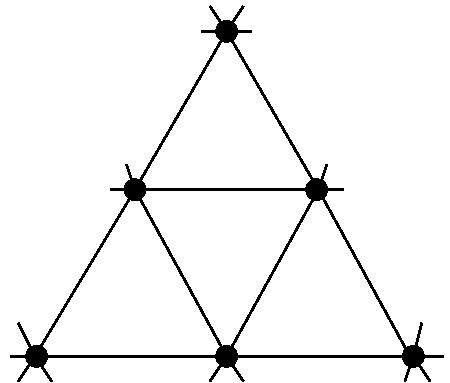
\includegraphics[width=0.4\linewidth]{Holyergraph.pdf}
\caption{Holyer's $H_{3,p}$ graph}
\end{figure}

The $\mathsf{FCP}$ version of the problem is to find the fewest number of triangles we must give in order for there to be a unique triangle partition. For example, in $H_{3,p}$ (Figure~\ref{fig:holyergraph}), once you specify one triangle in the partition, there is only one way to partition the graph in accordance with that triangle.

We claim $\mathsf{FCP}$ Triangle Partition is $\Sigma_2^P$-complete. We give a quick summary of Holyer's reduction which highlights the ideas we will use to show it is $\Sigma_2^P$-complete. 

\subsubsection{Holyer's Reduction for Triangle Partition}
%
% Fermi, do you think we need both paragraph version of summary and important properties?
%
% 
Holyer uses the graph $H_{3,p}$ (shown in Figure~\ref{fig:holyergraph}) to represent variables and literals. Each graph can only be partitioned in one of two ways. One way will correspond to a true setting, the other will correspond to a false setting. They called the two possible partitions the $T$-partition and the $F$-partition. 

\begin{figure}
\begin{minipage}{0.5\linewidth}
\centering
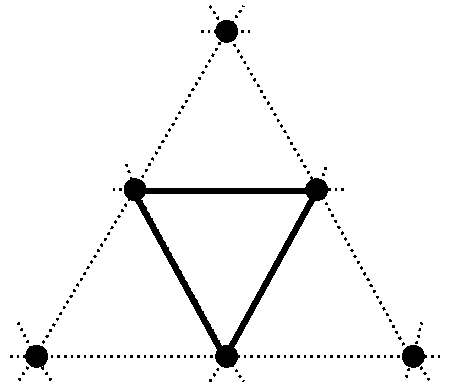
\includegraphics[scale=0.5]{Tpartition.pdf}
\label{fig:tpart}
\caption{$H_{3,p}$ partitioned like a $T$-partition. In a particular part of the graph, one triangle 'pointing down' specified.}
\end{minipage}
\hfill
\begin{minipage}{0.5\linewidth}
\centering
\label{fig:fpart}
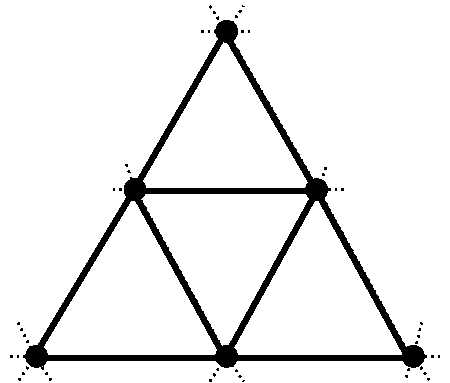
\includegraphics[scale=0.5]{Fpartition.pdf}
\caption{$H_{3,p}$ partitioned like an $F$-partition. In a particular part of the graph, three triangles 'pointing up' specified.}
\end{minipage}
\end{figure}

The authors also use the graphs to make clauses. They show a way to join three $H_{3,p}$ graphs such that exactly one of them will be $T$-partitioned. The three graphs will correspond to literals in the clause. Then they give a way to combine the literals with the variables such that if a literal is set to an $F$-partition, the corresponding variable must be set to either a $T$-partition (in the case where the literal is positive), or an $F$-partition (if the literal is negative). However, if the literal is a $T$-partition, then it does not matter what the variable is set to. 

In particular, there are three important properties of Holyer's reduction which we utilize:
\begin{enumerate}
\item We have variable and literal gadgets. These are graphs which can be partitioned in two possible ways. A graph is $T$-partitioned if it corresponds to setting that variable to true and $F$-partitioned otherwise.  
\item A clause gadget is a join between three literal gadgets. The clause gadget has a triangle partition if exactly one of the literals is $F$-partitioned.
\item A literal is joined with a variable. If the literal is $F$-partitioned, then there are two options:
\begin{itemize}
\item If the literal is the positive variable, then the variable must be $T$-partitioned.
\item If the literal is the negative variable, then the variable must be $F$-partitioned.
\end{itemize}
\end{enumerate}

If there exists a triangle partition of the graph, then each clause is satisfied by at least one literal. That literal gadget will be $F$-partitioned and it will cause the variable to take a particular partition, giving it its assignment. 

\begin{theorem}
$\mathsf{FCP}$ Triangle Partition is $\Sigma_2^P$-complete.
\end{theorem}

\begin{proof}
We refer the reader to \cite{holyer1981np}, \cite{colbourn1984complexity} for questions about notation. We reduce from $3\SAT$.

We let $f$ map instances of $3\SAT$ to Triangle Partition as in \cite{holyer1981np}. Suppose $c_{f(x)}$ is a minimal clue for the graph $f(x)$ (coming from the $3\SAT$ formula $x$). $c_{f(x)}$ consists of a set of triangles. Let 
\[ c_{f(x)} = L \cup V. \]
Where $L$ contains the triangles in the literal graphs, and $V$ contains the triangles in the variable graphs. 

\begin{claim}
Without loss of generality, $L$ contains triangles facing up (i.e, they correspond to an $F$-partition).
\end{claim}

The above claim follows from the fact that exactly one literal from each clause will be $F$-partitioned. If there is a triangle $t \in L$, which is facing down, is part of literal $l_c$ (in clause $c$). Then $c$ contains some other literal $l_c'$ which is $F$-partitioned. Exchanging the triangle $t$ for some upwards facing triangle in $l_c'$ decreases the number of triangles in $L$ which are facing down. We can apply this until we have no downward facing triangles in $L$. 

We then apply the following rule:
\begin{itemize}
\item Suppose $t \in L$ which faces up (corresponds to a literal which is an $F$-partition). $t$ is in some literal $l_c$ which represents the variable $x$. If $x$ is positive in $l_c$, then we exchange $t$ for some downward facing triangle in the variable graph for $x$. If $x$ appears negated in $l_c$, then replace $t$ by an upwards facing triangle in $x$.  
\end{itemize}

The above procedure ``transfers" the information from the literals to the variables. We know that an $F$-partitioned literal must be true in some clause. That particular variable will make the clause true, so we set the variable accordingly. Note that we no longer have a unique Triangle Partition corresponding t�o these clues, since if there is a clause which has more than one true literal, there are multiple ways to partition that clause. Let's call the transformed clue $c_{f(x)}'$. Note that $c_{f(x)}'$ is a clue for the same solution $c_{f(x)}$ is a clue for.

Now in order to make the clue for the $3\SAT$ formula, we say that if some triangle in the variable gadget for $x$ is downward facing (it makes the graph for $x$ $T$-partitioned), we let $x$ be true in $c_x$. If some triangle in the variable gadget for $x$ is upward facing (it makes the graph for $x$ $F$-partitioned), then we make $x$ be false in the clue, $c_x$. 

We need to show three things:
\begin{enumerate}
\item $c_x$ is a clue.
\item $c_x$ has a unique solution.
\item $c_x$ is minimal.
\end{enumerate}

1. We know $c_x$ must be a clue, since the transformed $c_{f(x)}$ had a clue. \\
2. Suppose $c_x$ has two satisfying assignments. Then if we partition the variable graphs according to the assignment, the partition is consistent with $c_{f(x)}'$. So the two assignments are consistent with $c_{f(x)}$. This is a contradiction.\\
3. Suppose $c_x$ is not minimal, .... AND stuck here.

\begin{comment}

We define $C_B'$ to be the following: we only consider solutions to Triangle Partition where in each clause, the first true literal is $F$-partitioned. We do this to remove the ambiguity of how to partition the graph into triangles in the clause gadget. $C_B'$ will be the set of clues corresponding to those solutions with clues only in the variable graphs $H_{3,p}$. 

Consider the following algorithm $M$ mapping instances of $C_B$ to $C_B'$. Suppose we are given a clue $c_x \in C_B$, consisting of a set of triangles. 
\begin{enumerate}
\item Suppose there is a triangle $t$ in a literal graph $l_c$ for some clause $c$. Suppose $t$ is pointing down. This means that $t$ specifies that the graph $l_c$ is $T$-partitioned. Then there must exists some other literal in the same clause which is $F$-partitioned. Let's call this literal graph $l_c'$. $M$ exchanges $t$ for a triangle in $l_c'$ which points upwards (corresponding to $l_c'$ being $F$-partitioned). 
\item Now that all clues in the clauses correspond to triangles which are $F$-partitioned in literal graphs, we exchange the triangles for a triangle in the variable graph which determines the assignment of the variable.
\end{enumerate}

We define $g: C_B' \rightarrow C_A$ to map triangles in variable graphs to the corresponding assignment. So if a variable graph $x$ contains a triangle pointing upwards (corresponding to an $F$-partition), then we let $x$ be false. If the variable graph contains a triangle pointing downwards (corresponding to a $T$-partition), then we let $x$ be true. 

We check $g$ satisfies the requirements for a Special Subset Clue Reduction.
\begin{itemize}
\item $g$ is surjective. This is true because the variable assignments correspond to variable gadget partitions.
\item $g$ is a bijection on solutions. Once the variable graphs are partitioned we force the first true literal to be $F$-partitioned. 
\item Because we are mapping individual triangles, subsets are preserved. If $g(c) \subset S$, then $g^{-1}(S)$ presents a full triangle partition from $C_B'$, so $c \subset g^{-1}(S)$. 
\item We are projecting certain triangles to variables, so there is at most one variable per triangle. In minimal clue sets, we will need exactly one variable per triangle.
\end{itemize}
\end{comment}
\end{proof}

\subsection{Latin Squares}

The Latin Squares problem is the following:
\begin{quote}
\textbf{Instance}: An $n \times n$ grid, with some entries filled in with the numbers $1$ to $n$.\\
\textbf{Question}: Can we fill in the remainder of the grid with numbers from $1$ to $n$ while enforcing that no row or column repeat a number?
\end{quote}
The problem was shown to be $\NP$-complete by Colbourn \cite{colbourn1984complexity}. Here, we study its  $\mathsf{FCP}$ version, which asks what is the fewest number of entries that must be filled in so the Latin Square becomes uniquely solvable. We claim this problem is $\Sigma^P_2$-complete. 

\subsubsection{Colbourn's Reduction for Latin Squares:}
We give a quick summary of Colbourn's main ideas which will help the reader understand the $\Sigma^P_2$-completeness reduction. There are two main steps in his proof. In the first, Colbourn shows that completing partial Latin Squares is equivalent to partitioning tripartite graphs into triangles, a problem similar to the one in section \ref{S:TP} which is shown to be $\NP$-complete. In the second step, the authors use embedding techniques to reduce triangle partitions of tripartite graphs to Latin Square completion. 

We say a tripartite graph $G = (V_1 \cup V_2 \cup V_3, E)$ is \emph{uniform} if any vertex $x \in V_1$ (symmetrically $V_2, V_3$) has the following property: it has the same number of neighbors on the other two parts of the partition.  Colbourn \cite{colbourn1984complexity} argues that in order to decide if a triangle partition exists on a tripartite graph it suffices to consider the cases where the graph is uniform. A tripartite graph with a triangle partition must be uniform. 

Throughout this section we refer to the entry on the $i$-th row and $j$-th column of a Latin Square as $L(i,j)$. The authors introduce the concept of a defect graph $G(P)$, a tripartite graph that has a triangle partition if and only if its originating Latin Square $P$ is completable. 

\begin{definition}
Suppose we are given a partial Latin Square $P$ of order $n$. The defect graph $G(P) = (V,E)$ of $P$ is the graph whose vertex set is given by $$\{ r_i | \text{ row } i \text{ contains an empty square} \} \cup \{ c_j | \text{ column } j \text{ contains an empty square} \} $$
$$ \cup \{ e_k | \text{ element } k\text{ appears less than } n \text{ times } \} .$$ 

The edge set of $G(P)$ is defined as follows: 

\begin{itemize}
	\item If $L(i,j)$ is blank, then we add an edge between $r_i$ and $c_j$. 
	\item If row $i$ does not have item $k$ then we add an edge between $r_i$ and $e_k$. 
	\item If column $j$ does not have item $k$ then we add an edge between $c_j$ and $e_k$.
\end{itemize}
\end{definition}

\begin{figure}
\centering
\label{fig:LStoTrianglePartitionExample}
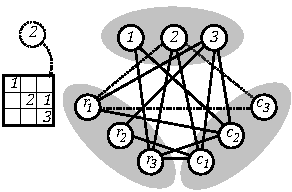
\includegraphics[width=0.5\linewidth]{latinsquare_to_triangle_part_2.pdf}
\caption{Example of a $3\times 3$ Latin Square and its defect graph. We highlight the correspondence between a triangle in the graph and an entry of the grid.}
\end{figure}

Colbourn \cite{colbourn1984complexity} shows the following lemma: 
\begin{lemma}\label{TP:lemma}
A partially completed Latin Square $P$ has a valid solution if and only if its defect graph $G(P)$ has a triangle partition. 
 \end{lemma}
 
The authors show a modification of Holyer's proof that Triangle Partition is $\NP$-complete to show that finding a triangle partition of a tripartite graph is also $\NP$-complete. 

\begin{lemma}\label{TPTG:lemma} 
$\mathsf{FCP}$ Triangle Partition of Tripartite Graphs is $\Sigma_2$-complete. 
\end{lemma}

\begin{proof}
We use the same modifications that Colbourn uses to show the problem is $\NP$-complete. Note that Holyer's building blocks, $H_{3,p}$, are 3-colorable (i.e. tripartite) if and only if $p \equiv 0 (\mod 3)$. So in the modified proof, $p$ is chosen so that it always satisfies this property. Hence, the graph will always be tripartite. Moreover, when the partitions are decided to maintain vertices of the same color. This does not alter the proof in the previous section, but it guarantees that the graph remains 3-colorable. 
\end{proof} 

Next, Colbourn shows the reduction from the problem of finding triangle partitions in tripartite graphs to Latin Squares completion by introducing the concept of a Latin Framework. 

\begin{definition} 
Let $G = (V, E)$ be a tripartite graph with partition $V = V_1 \cup V_2 \cup V_3$ and $V_1 = \{r_1,...,r_x\}$, $V_2 = \{c_1,...,c_y\}$ and $V_3 = \{e_1,...,e_z\}$. A \emph{Latin Framework} of such a tripartite graph, denoted as $LF(G;r,s,t)$ is an $r \times s$ array whose entries can be empty or contain one of the numbers from $\{1, ... ,t \}$, with each row and column containing a number at most once. Given $G$, we build $LF(G;r,s,t)$ according to these rules: 

\begin{itemize}
	\item If $(r_i, c_j) \in E$, then the $(i,j)$ entry of $LF(G;r,s,t)$ is empty. Otherwise it contains a number from $\{1,2,...,t\}$. 
	\item If $(r_i, e_k) \in E$ then row $i$ of $LF(G;r,s,t)$ does not contain element $k$. 
	\item If $(c_j, e_k) \in E$ then column $j$ of $LF(G:r,s,t)$ does not contain element $k$. 
\end{itemize}
\end{definition}

If all dimensions of the Latin Framework are equal, $G$ is the defect graph of $LF(G;r ,r, r)$. Therefore, it suffices to show that arbitrary Latin Frameworks can be reduced to this case with a small blowup in size. Consider the following Lemma, shown by Colbourn: 

\begin{lemma}
For an $n$-vertex uniform tripartite graph $G$, there is a Latin Framework $LF(G;n,n,2n) L$. 
\end{lemma} 

\begin{proof}
Construct the following $n \times n$ array $L$. If $(r_i, c_j) \in E$, leave $L(i,j)$ blank. Otherwise, Let $L(i,j) = 1 + n + ((i+j) \mod n)$. Then $L$ is a Latin Framework with the claimed dimensions since we are using numbers from $1$ to $2n$. 
\end{proof}

Note that we can always create an $n$-vertex uniform graph by simply adding isolated vertices to each partition until they have the same size. This allows us to assume without loss of generality that our graph will have $n$ vertices on each partition. Colbourn uses the following embedding technique, whose proof we omit, to show that any $n$-vertex uniform tripartite graph $G$ has a Latin Framework $LF(G;2n,2n,2n)$ which can be constructed in polynomial time. 

\begin{lemma}
Let $L$ be an $LF(G;r,s,t)$ for a uniform tripartite graph $G$. Let $R(k)$ be the number of times element $k$ appears in $L$ plus half the degree of $e_k$ in $G$. Then, whenever $R(k) \geq r + s - t$ for all $1 \leq k \leq t$, $L$ can be extended to an $LF(G;r, s+1, t) L'$ in which $R'(k) \geq r + (s+1) - t$ for all $1 \leq k \leq t$. 
\end{lemma} 

Once we have a Latin Framework $LF(G;n, n, 2n)$ we can add columns until we have $2n$ of them. We can then take the transpose of the array and add rows until we get $2n$ of them as well. This allows us to construct Latin Frameworks of equal dimensions given $n$-vertex uniform tripartite graphs. 

\begin{theorem}
$\mathsf{FCP}$ Latin Squares is $\Sigma_2^P$-complete.
\end{theorem}

\begin{proof}
We do this via a general FCP reduction from $\mathsf{FCP}$ Triangle Partition of Tripartite Graphs.

Given a tripartite graph $G$, we first check whether or not it is uniform. If it is not uniform, then there does not exist a triangle partition as argued by Colbourn. If it is uniform, we can write down a Latin Framework $LF(G;2n,2n,2n)$ in polynomial time \cite{colbourn1984complexity}. This Latin Framework is constructed so that $G$ is the defect graph of $LF(G;2n,2n,2n)$. We then map via $f$ instances of defect graphs $G$ to partial Latin Squares. This map is bijective as stated in lemma \ref{TP:lemma}. There is a triangle partition of $G$ if and only if we can complete the partial Latin Square $LF(G;2n,2n,2n)$. This implies that the triangle partitions of a defect graph $G$ are in one to one correspondence with the solutions to their Latin Squares. 

The mapping on clue sets $g$ sends Latin Squares clues $L(i,j) = k$ to triangles with vertices $(i,j,k)$ on different parts of the partition. 
\begin{itemize}
	\item $g$ is surjective. It maps a Latin Squares clue to a valid Triangle Partition clue
	\item $g$ is bijective on solutions. By construction, the triangle takes into account the row, column and number of the clue.
	\item $g$ preserves subsets. We are mapping filled squares to triangles individually.
	\item $g$ preserves the sizes of clues. Again, it maps filled squares to triangles individually. 
\end{itemize}

\end{proof}

\subsection{Sudoku}

The Sudoku problem is the following: 

\begin{quote}
\textbf{Instance}: A board of $n^2 \times n^2$ numbers in the range of $1$ to $n^2$, divided into $n^2$ blocks of size $n \times n$.\\
\textbf{Question}: Can we fill up the remaining squares with numbers in the range $1$ to $n^2$ such that each row, column and $n \times n$ block does not have repeated numbers?
\end{quote}

The $\mathsf{FCP}$ version of the problem asks for the least number of additional numbers we must give in order to have the Sudoku be uniquely solvable. We will show this problem is $\Sigma_2^P$-complete by providing a General Clue Reduction from $\mathsf{FCP}$ Latin Squares. 

Before showing the main result of this section, we will exhibit a particular way to fill a Sudoku puzzle. Next, we will show how this particular solution can be used to explicitly map instances of Sudoku to instances of Latin Squares. For simplicity, throughout this argument we will be using numbers in the range $0$ through $n^2 - 1$. This does not change the problem. The $n^2$ symbols in Sudoku have no relation to each other, only their equality or inequality. We will refer to the entry on the $i$-th row and $j$-th column of a Sudoku puzzle as $S(i,j)$.

\begin{proposition}[\cite{takayuki2003complexity}]
\label{prop:s_0}
Let $S_0$ be defined as
\[ S_0 (i,j) = ((i \mod n) n + \lfloor i/n \rfloor + j) \mod n^2 \]
Then $S_0$ represents a solution to an order $n$ Sudoku.
\end{proposition}

The proof of the Proposition~\ref{prop:s_0} appears in \cite{takayaki2003complexity}. We show an example construction for $n=3$, the classic Sudoku puzzle.

\begin{figure}
\centering
\label{fig:s_0}
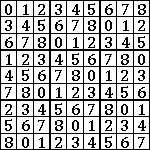
\includegraphics[width=0.6\linewidth]{sudoku_s_0.pdf}
\caption{Complete $S_0$ Sudoku for $n = 3$. The construction is defined in Proposition~\ref{prop:s_0}.}
\end{figure}

\begin{lemma}[\cite{takayuki2003complexity}]
\label{lem:sudoku_reduction}
Let $S$ be a Sudoku instance of order $n$ such that
\begin{displaymath}
S(i,j) = \left\{
\begin{array}{lr}
\perp & : (i,j) \in B\\
S_0 (i,j) & : \text{otherwise}
\end{array}
\right.
\end{displaymath}
where $B = \{ (i,j) | i < n \text{ and } (j \equiv 0) \mod n \}$. Let $S'$ be the Sudoku obtained by filling in the blanks of $S$. Then $S'$ is a correct Sudoku solution if and only if the following conditions hold:
\begin{itemize}
\item For any $(i,j) \in B$, $S'(i,j) \equiv 0 \mod n$
\item A square $L$ defined by $L(i, j/n) = S'(i,j)/n$ for all $(i, j) \in B$ is a complete Latin Square.
\end{itemize}
\end{lemma}

The proof of Lemma~\ref{lem:sudoku_reduction} is also in \cite{takayuki2003complexity}. Figure~\ref{fig:latinsquare_to_sudoku} shows how the Latin Square corresponds to certain sections of the Sudoku puzzle for $n=3$. The three columns of the Latin square are mapped to the parts of columns of the Sudoku. In the mapping,the values are scaled by $n$. 

\begin{figure}
\centering
\label{fig:latinsquare_to_sudoku}
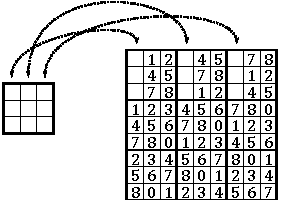
\includegraphics[width=0.7\linewidth]{latinsquare_to_sudoku.pdf}
\caption{Latin square taken from parts of $S_0$.}
\end{figure}

Lemma ~\ref{lem:sudoku_reduction} gives us the reduction from Latin Square completion to Sudoku completion. Given a Latin Square, we can create a Sudoku instance $S$ from the lemma. This is the reduction from \cite{takayuki2003complexity}.

\begin{lemma} 
$\mathsf{FCP}$ Sudoku is $\Sigma_2^P$-complete.
\end{lemma}

\begin{proof} 
We will show a General Clue Reduction via $\mathsf{FCP}$ Latin Squares. We use the injective map from instances of Latin Square to instances of Sudoku described in Lemma~\ref{lem:sudoku_reduction}. Let $C_B$ be the set of set of clues of Sudoku. We define $g$, by mapping a clue of Sudoku indicating that location $(i,j)$ contains $S(i,j)$ to the clue saying that the $(i, j/n)$ position of the Latin Square is $S(i, j)/n$. 
\begin{itemize}
\item $g$ is surjective. Each Latin Square clue came from a clue of Sudoku.
\item $g$ is bijective on solutions. Each solution to Sudoku gives a solution to Latin Squares, and the solution is unique since all other numbers are parts of the instance. 
\item $g$ maps each clue to another clue. So subsets are always preserved: $c \subset c' \iff g(c) \subset g(c')$. 
\item $g$ maps each clue to one clue. Therefore the size of a clue set is preserved. 
\end{itemize}
Therefore, $\mathsf{FCP}$ Sudoku is $\Sigma_2^P$-complete. 
\end{proof}

\section{$\mathsf{FCP}$ Versions of Easy Problems}
\label{sec:easyproblems}

We would like to be able to understand what happens to problems in general when their $\mathsf{FCP}$ versions are asked.

\subsection{Connection to Counting Problems}

For any search problem, the related counting problem asks for the number of valid solutions. We suspect that problems in $\mathsf{P}$ with $\sharp \mathsf{P}$-hard counting problems also have hard $\mathsf{FCP}$ versions.

\subsection{$\mathsf{FCP}$ 2SAT} 


In this section, we consider the $\mathsf{FCP}$ version of the 2-satisfiability ($2SAT$) problem. The problem, which gives a 2-CNF Boolean formula and asks for a satisfying assignment, has a known polynomial time solution. However, the \emph{counting} version of the problem is a well-known $\sharp \mathsf{P}$-complete problem. In this section, we show $\mathsf{FCP}-2SAT$ is $\mathsf{NP}$-complete, lending credence to the idea that $\sharp \mathsf{P}$-hardness and $\mathsf{FCP}$-hardness are related. Formally, $\mathsf{FCP}-2SAT$ is formulated as follows.

\begin{quote}
\textbf{Instance}: A 2-CNF Boolean formula $\phi$ on variables $x_1, ..., x_n$. \\
\textbf{Question}: Does there exist a setting of $k$ variables so that the remaining formula is uniquely satisfiable?
\end{quote}

\begin{proposition}
$\mathsf{FCP} 2SAT$ is in \NP.
\end{proposition}

\begin{proof}
The clue of size $k$ is the certificate. Since $2SAT$ can be satified in polynomial time, we can check whether there is a unique solution in polynomial time.
\end{proof}

\begin{theorem} 
$\mathsf{FCP} 2SAT$ is \NP-hard.
\end{theorem}

We reduce from the NP-hard problem of determining whether a graph has an independent dominating set of size at most $k$ (MIDS). The problem gives a graph $G = (V,E)$ and asks for the smallest subset of vertices $S \subseteq V$ such that $S$ is an independent dominating set and $|S| \leq k$. In other words, such a set $S$ has the property that every vertex has a vertex in $S$ adjacent to it (dominated), and does not include any vertex pairs $u$ and $v$ where $(u,v)$ is an edge in the graph (independent). \\

\noindent\textbf{Problem:} Given a graph $G = (V, E)$. Does there exist $S \subset V$, with $|S| \leq k$ such that 
\begin{itemize}
\item $\forall v \in V$, either $v \in S$ or $(u, v) \in E$, $u \in S$ 
\item $u, v \in S$ implies that there is no edge between $u$ and $v$. 
\end{itemize}

\begin{figure}
\label{fig:2SATgraph}
\begin{minipage}{0.5\linewidth}
\centering
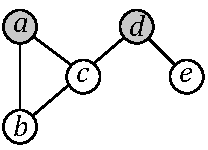
\includegraphics{2satreduct.pdf}
\end{minipage}
\hfill
\begin{minipage}{0.5\linewidth}
\centering
\begin{equation}
\begin{split}
(\neg a \vee \neg b)&\wedge(\neg a \vee \neg c) \\ \wedge(\neg b \vee \neg c) &\wedge (\neg c \vee \neg d) \\ \wedge(\neg d \vee \neg e)
\end{split}
\end{equation}
\end{minipage}
\caption{Reduction from Minimum Independent Dominating Set to $\mathsf{FCP} 2\SAT$.}
\end{figure}

The reduction works as follows. For each edge $(u,v)$, we add the constraint $(\neg u \vee \neg v)$ to the 2SAT formula. We claim that a clue set for the resulting 2SAT formula where all clues set variables to be true can be transformed into an independent dominating set of size $k$. For the backwards direction, we claim that an independent dominating set of size $k$ can be turned into a clue set of size $k$. 

%
%We claim that a clue set for the resulting 2SAT formula consists of a setting of $k$ variables to be true, and that the variables in the clue correspond to a minimum independent dominating set. For the other direction, we claim that a minimum independent dominating set gives us a minimum clue set for the 2SAT formula, by simply setting all the variables corresponding to vertices in the set to be true.

In order to restrict our attention to clues that set variables to be true, we need the following lemma.

\begin{lemma} Given a set of clues of size $k$ with $k_f > 0$ variables set to false, there exists another set of clues of size at most $k$ with strictly fewer than $k_f$ variables set to false.
\end{lemma}

\begin{proof} 
Consider a variable $x_i$ set to be false. Consider its set of neighbors $N(x_i)$, guaranteed to be non-empty via construction. First, consider the case where $N(x_i)$ contains nodes set to true. For each of the nodes $v \in N(x_i)$ that are set to true, a clue must either say that $v$ is true, or there must be a clue that implies that $v$ is true. No matter what, we can either remove $x_i$ or replace $x_i$ with a clue that one of its neighbors are true (CHECK THIS). It remains to consider the case where all the neighbors of $x_i$ are set to false. In this case, we can switch the clue that $x_i$ is set to false with a clue that $x_i$ is set to true, which will imply that all of its neighbors are false.
\end{proof}

Now, we show that a clue assignment gives an independent dominating set of the same size. Suppose we have a clue assignment of size at most $k$. We first apply the lemma above repeatedly until there are no false clues. So if we have a variable that is part of the clue, it is set to be true and implies all of its neighbors are false. Thus, we get independence because we cannot have two adjacent variables set to true. We have a dominating set as well, since if there exists a vertex where no neighbor is a clue, then we cannot possibly know that any neighbors are set to true (since clues can only imply that other vertices are false), and since true variables are the only ones that give implications, we cannot know what this vertex is. 

Now we show that an independent dominating set gives a clue assignment of the same size. Suppose we have a minimum independent dominating set. If we set each variable in the minimum independent dominating set to be true, then we know due to the fact that it is a dominating set that every variable will be implied. So we know that this is a valid clue set.

Ideally, we would like to generalize what we've shown above. One particular question is whether the $\mathsf{FCP}$ versions of problems with polynomial time algorithms have a better upper bound than $\Sigma_2$. In general the answer is no. Consider the following example:
\[ L = \{ \phi' = \phi \vee \left( \bigwedge_i x_i \right) | \phi \text{ is a Boolean formula }\} \]
Clearly, $L \in P$. Since on each input, we check whether the Boolean formula takes the following form, and if so, we accept. The clause with all variables being $1$ indicates that the formula has a satisfying assignment. In addition, the search problem for finding a satisfying assignment also has a polynomial time algorithm. We simply set all variables to $1$. However, what happens to the $\mathsf{FCP}$ version?

$\mathsf{FCP} L$ 
\begin{quote}
\textbf{Instance}: a Boolean formula $\phi \vee \left( \bigwedge_i x_i\right)$, along with a $k$.\\
\textbf{Question}: Is there a partial assignment of at most $k$ variables such that the remaining formula is a unique satisfying solution?
\end{quote}

\begin{proposition}
$\mathsf{FCP} L$ is co\NP-hard.
\end{proposition}

\begin{proof}
We can reduce from $\overline{SAT}$. 
\begin{align}
\phi \in \overline{SAT} &\leftrightarrow \forall x \phi(x) = 0 \\
				    & \leftrightarrow \langle (\phi \wedge \overline{z}) \vee \left(z \wedge \bigwedge_i x_i \right), 0 \rangle \in \mathsf{FCP} L
\end{align}
\end{proof}

Alternatively, we could look at another contrived language:
\[ L' = \{ \phi' = (\phi \wedge \overline{z}) \vee z | \phi \text{ is a Boolean formula and $z$ does not appear in $\phi$} \} \]
So $L' \in P$ and the search problem also has a polynomial time algorithm. However, it seems like $\mathsf{FCP} L'$ should be able to analyze what happens inside $\phi$. 

\begin{proposition}
$\mathsf{FCP} L'$ is $\Sigma_2$-complete. 
\end{proposition}

\begin{proof}
We reduce from $\mathsf{FCP} SAT$. If $\phi$ has a partial assignment of size at most $k$ with a unique solution, then $\phi' = (\phi \wedge \overline{z}) \vee z$ has a partial assignment of size at most $k+1$ with a unique solution. We simply add the assignment for variable $z$. 

If $\phi$ has no satisfying assignment, then $\phi'$ requires $n$ clues for a partial assignment with a unique solution. If $\phi$ has a partial assignment, but it requires more than $k$ clues, then if $\textbf{x}$ is a particular satisfying assignment to $\phi'$, if $z  \in \textbf{x}$, then $\textbf{x}$ needs at least $n$ solutions to be specified, if $\overline{z} \in \textbf{x}$, then we must specify $\overline{z}$ in the clue, and by assumption we must specify more than $k$ variables. Therefore, if $\phi$ needs more than $k$ clues, $\phi'$ will need more than $k+1$ clues. 
\end{proof}

\subsection{What can we say about easy languages?}

NEED TO FORMALIZE THIS A BIT MORE.

We can say something about a particular set of easy problems. 
\begin{proposition}
Suppose $A$ in a search problem with a polynomial time algorithm. Furthermore, suppose $x$ is an instance of $A$. If $c$ is some clue for $x$ and $x \cup c$ is another instance of $x$, then $\mathsf{FCP} A \in \NP$. 
\end{proposition}

\begin{proof}
The certificate is the clue, along with the solution. We only need to specify that the clue is the required size, the solution corresponds to the clue, and that there is a unique solution. We do this by showing by asking whether $x \cup c \cup \{ c' \}$ has a solution for each possible additional clue $c'$ (for which there are polynomially many). If we can find more than one solution, we reject. If there is only one solution, we accept. Since $x \cup c \cup \{ c' \}$ is an instance to $A$, and $A$ has a polynomial time algorithm, we can verify that $c$ is a clue with a unique solution in polynomial time.
\end{proof}

We know that many polynomial time problems which we care about satisfy the above self-reducibility property. These include 2SAT, Horn-satisfiability, and matching. The languages $L$ and $L'$ do not satisfy the above properties.

\section{Conclusion}
\label{sec:conclusion}


\bibliography{references}
\bibliographystyle{splncs}
\end{document}
